
\section{统计}

\begingroup
\def\pgfplotsmanualcurlibrary{statistics}
\tikzset{external/figure name/.add={}{statistics_}}

\begin{pgfplotslibrary}{statistics}
    本库提供用于统计的绘图处理器。
\end{pgfplotslibrary}


\subsection{箱线图}
\label{sec:boxplots}

\begingroup

\pgfkeysgetvalue{/pgfmanual/gray key prefixes}\oldgraykeyprefixes
\pgfkeys{
    /pdflinks/search key prefixes in/.add={}{,/pgfplots/boxplot/},
    /pgfmanual/gray key prefixes/.add={/pgfplots/boxplot/,}{},
}%

箱线图是一维分布的可视化。它们提供分布特征的快速概览。箱线图本质上是一维的；
它们仅使用第二个坐标轴将多个箱线图并排放置。

\PGFPlots{} 支持两种相关的绘图处理器：|boxplot| 与 |boxplot prepared|。
|boxplot| 处理器以一维样本为输入，计算 |median|、|lower quartile|、
|upper quartile|、|lower whisker| 与 |upper whisker|，并使用
|boxplot prepared| 处理器可视化结果。|boxplot prepared| 处理器在输入上期望所有
所需值并将其可视化。


\subsubsection{预备箱线图与通用选项}

先讨论 |boxplot prepared| 处理器；其所有自定义同样适用于 |boxplot|。

\begin{plottype}[/pgfplots]{boxplot prepared=%
    \textcolor{black}{\normalfont\marg{options with {\normalfont\texttt{boxplot/}} prefix}}%
}
    |boxplot prepared| 接受若干描述所需统计量的键--值对，以及一个离群点坐标流作为
    输入，并绘制箱线图。
    %
\begin{codeexample}[]
\begin{tikzpicture}
\begin{axis}
    \addplot+ [
        boxplot prepared={
            lower whisker=5,
            lower quartile=7,
            median=8.5,
            upper quartile=9.5,
            upper whisker=10,
        },
    ] table [row sep=\\,y index=0] {
        data\\ 1\\ 3\\
    };
\end{axis}
\end{tikzpicture}
\end{codeexample}
    %
    \noindent 上例展示了 |boxplot prepared| 的主要思想：每个所需量都必须用
    键--值语法显式提供。后面的坐标流可以为空；其中的所有坐标都被视为离群点。
    它们以散点图绘制。

    箱线图产生两个坐标：一个属于输入数据（例如 |median|），另一个仅用于绘图。
    两者都会更新界限。对于显示输入数据的坐标轴（本例为 $x$，另见 |draw direction|）
    这很清楚，但应注意，另一条坐标轴的界限与缩放参数将与其他任何图一样选取。
    箱体的延伸默认略小于一个单位（参见 |box extend|）。因此，可能需要为剩余
    坐标轴调整界限或缩放参数：
    %
\begin{codeexample}[]
\begin{tikzpicture}
\begin{axis}[
    y=1.5cm,
]
    \addplot+ [
        boxplot prepared={
            lower whisker=5,
            lower quartile=7,
            median=8.5,
            upper quartile=9.5,
            upper whisker=10,
        },
    ]
        table [row sep=\\,y index=0] {
        data\\ 1\\ 3\\
    };
\end{axis}
\end{tikzpicture}
\end{codeexample}
\end{plottype}

若将多个使用 |boxplot prepared| 处理器的图放入同一坐标轴，它们会通过
|draw position| 的默认值自动并排放置：

\begin{pgfplotskey}{boxplot/draw position=\marg{axis unit to place box} (initially 1+\textbackslash plotnumofactualtype)}
    |draw position| 键决定如何选择箱线图的位置，即可自由选择的坐标轴单位。

    初始配置将第一个箱线图放在 $y=1$，后续的放在下一个整数。
    %
\begin{codeexample}[]
\begin{tikzpicture}
\begin{axis}
    \addplot+ [
        boxplot prepared={
            lower whisker=42, lower quartile=45,
            median=47,
            upper quartile=47.5, upper whisker=48,
        },
    ] table [row sep=\\,y index=0] { 40\\ 34\\ 56\\ };

    \addplot+ [
        boxplot prepared={
            lower whisker=36, lower quartile=39,
            median=40,
            upper quartile=41, upper whisker=43,
        },
    ]
        % no outliers:
        coordinates {};

    \addplot+ [
        boxplot prepared={
            lower whisker=41, lower quartile=44,
            median=45,
            upper quartile=46, upper whisker=47,
        },
    ] coordinates {(0,35) (0,55)};
\end{axis}
\end{tikzpicture}
\end{codeexample}
    %
    上例在同一坐标轴中展示三个箱线图。注意，它们使用默认设置对齐。

    前 $N$ 个 |boxplot|（或等价的 |boxplot prepared|）放在坐标 $1,2,3,\dotsc,N$
    处，这使得分配刻度标签很简单：使用 |ytick=data|，或 |ytick=1,2,3| 配合
    |yticklabels|：
    %
\begin{codeexample}[]
\begin{tikzpicture}
\begin{axis}[
    ytick={1,2,3},
    yticklabels={Group A, Group B, Group C},
]
    \addplot+ [
        boxplot prepared={
            lower whisker=42, lower quartile=45,
            median=47,
            upper quartile=47.5, upper whisker=48,
        },
    ] table [row sep=\\,y index=0] { 40\\ 34\\ 56\\ };

    \addplot+[
        boxplot prepared={
            lower whisker=36, lower quartile=39,
            median=40,
            upper quartile=41, upper whisker=43,
        },
    ] coordinates {};

    \addplot+[
        boxplot prepared={
            lower whisker=41, lower quartile=44,
            median=45,
            upper quartile=46, upper whisker=47,
        },
    ] coordinates {(0,35) (0,55)};
\end{axis}
\end{tikzpicture}
\end{codeexample}

    \noindent 可以使用 |draw position=\thisrow|\meta{colname} 从某输入表读取
    |draw position|。此时将使用最后遇到的数据行（当然，此说明仅在存在数据流时
    有用）。

    虽然 |draw position| 的默认选择有望覆盖最常见用例，但如果希望单独放置特定
    箱线图，也可以为其自定义值：
    %
\begin{codeexample}[]
\begin{tikzpicture}
\begin{axis}[
    boxplot/draw direction=y,
]
    \addplot+ [boxplot prepared={
        lower whisker=2.5, lower quartile=4,
        median=8.5, upper quartile=12,
        upper whisker=15},
    ] coordinates {};
    \addplot+ [boxplot prepared={
        lower whisker=2.5, lower quartile=4,
        median=8.5, upper quartile=12,
        upper whisker=15},
    ] coordinates {};
    \addplot+ [boxplot prepared={draw position=5,
        lower whisker=2.5, lower quartile=4,
        median=8.5, upper quartile=12,
        upper whisker=15},
    ] coordinates {};
\end{axis}
\end{tikzpicture}
\end{codeexample}
    %
    \noindent 本例前两个图使用默认 |draw position|。由于它使用图索引 $+1$，
    它们分别放在 $x=1$ 与 $x=2$（因 |draw direction=y| 而使用 $x$）。第三个图
    有 |draw position=5|，绘制在 $x=5$。

    注意，若为一个图分配 |draw position|，可能还需要调整后续所有图，因为
    \PGFPlots{} 不会自动检测冲突。
\end{pgfplotskey}

\noindent 前面的例子从输入流的 $y$ 坐标读取离群点数据流：对于 |\addplot table|，
我们显式写了 |y index=0|；对于 |\addplot coordinates|，我们使用
|(0,35) (0,55)|，其中 $x$ 分量被忽略。此默认可通过 |boxplot/data| 键更改。

\begin{pgfplotskey}{boxplot/data=\marg{expression} (initially y)}
    告知 |boxplot| 如何获取其数据。通常做法是提供一个数学 \meta{expression}，
    它依赖于 |\addplot| 语句提供的数据。例如，若使用 |\addplot expression|，
    \meta{expression} 可依赖 |x|、|y| 或 |z|。对于 |\addplot table| 输入例程，
    \meta{expression} 可使用 |\thisrow|\marg{colname} 访问指定列中当前活动的
    表行。

    也可以避免调用数学解析器。改为使用
    \declareandlabel{boxplot/data value}|=|\marg{value}。这里，\meta{value}
    应为数值常量。

    初始配置使用通常成为最终 |y| 坐标的值作为输入（更准确地说，初始值为
    |data value=\pgfkeysvalueof{/data|\allowbreak| point/y}|）。
\end{pgfplotskey}

\begin{pgfplotskey}{boxplot/data filter/.code={\marg{code}} (initially empty)}
    允许用户安装过滤器。该过滤器的工作方式与其他过滤器非常相似。
    %
\begin{codeexample}[]
\pgfplotsset{
    only if/.style args={entry of #1 is #2}{
        /pgfplots/boxplot/data filter/.code={
            \edef\tempa{\thisrow{#1}}
            \edef\tempb{#2}
            \ifx\tempa\tempb
            \else
                \def\pgfmathresult{}
            \fi
        }
    }
}

% 'data.dat' contains
% v     set
% 0.1   a
% 0.2   a
% 0.3   a
% 0.8   b
% 0.9   b
% 1.0   b

\begin{tikzpicture}
\begin{axis}[
    boxplot,
    table/y=v,
    boxplot/draw direction=y,
]
 \addplot table[only if={entry of set is a}]{data.dat};
 \addplot table[only if={entry of set is b}]{data.dat};
\end{axis}
\end{tikzpicture}
\end{codeexample}
\end{pgfplotskey}

\begin{pgfplotskeylist}{%
    boxplot/lower whisker=\marg{value} (initially auto),
    boxplot/lower quartile=\marg{value} (initially auto),
    boxplot/median=\marg{value} (initially auto),
    boxplot/upper quartile=\marg{value} (initially auto),
    boxplot/upper whisker=\marg{value} (initially auto),
    boxplot/average=\marg{value} (initially empty)%
}
    这些键构成受支持的统计量。通常，箱线图会使用除 |average| 外的每一个。

    \meta{value} 的任何数值将原样使用。这对 |boxplot prepared| 与 |boxplot|
    都成立。

    空的 \meta{value} 会禁用相应的键：其关联可视化将被省略。这是 |average|
    的默认值。

    值 |auto| 告知 \PGFPlots{} 将该统计量纳入 |boxplot| 施加的自动计算。
    它对 |boxplot prepared| 无关紧要（在那里它本质上等同于空的 \meta{value}）。

    各值的定义如下。假设我们有某分布的给定样本，记为 $x_1,\dotsc,x_N$，并假设
    值已排序，$x_1 < \dotsb < x_N$（顺便说一句，这对 |boxplot| 并非要求）。
    对任意实数 $p$，$0\le p\le1$，“$p$ 分位数”（或 $p$ 百分比）定义为
        \[
            x_p :=
                \begin{cases}
                     x_{N \cdot p}
                        & \text{if $N \cdot p$ is an integer number}\\
                    \frac{1}{2} (x_{\lfloor N p \rfloor} + x_{\lceil N \cdot p \rceil})
                        & \text{if $N \cdot p$ is not an integer.}
                \end{cases}
        \]
    %FIXME : this is not as in textbooks! BUG in the computation!?

    |median| 是输入数据的 $0.5$ 分位数：一半的点小于中位数，一半的点大于中位数。

    |lower quartile| 是输入数据的 $0.25$ 分位数。

    |upper quartile| 是输入数据的 $0.75$ 分位数。

    |lower whisker| 是大于 |lower quartile|~$-1.5 \cdot \text{IQR}$ 的最小数据值，
    其中 $\text{IQR}$ 为“四分位距”，即 |upper quartile| 与 |lower quartile| 之差。

    |upper whisker| 是小于 |upper quartile|~$+1.5 \cdot \text{IQR}$ 的最大数据值。

    |average| 是样本均值。|boxplot| 在默认配置下省略它。将其设为 |auto| 以启用
    自动计算。
\end{pgfplotskeylist}

\begin{pgfplotskey}{boxplot/draw direction=\mchoice{x,y} (initially x)}
    由于 |boxplot| 本质上是一维的，它可沿 $x$ 轴或 $y$ 轴可视化。

    默认配置使用上面看到的 $x$ 方向。

    另一种选择 $y$ 让箱体及其须沿 $y$ 轴延伸，并将多个箱线图沿 $x$ 轴堆叠：
    %
    % FIXME : eliminate opacity=0 here!
\begin{codeexample}[]
\begin{tikzpicture}
\begin{axis}[
    boxplot/draw direction=y,
    x axis line style={opacity=0},
    axis x line*=bottom,
    axis y line=left,
    enlarge y limits,
    ymajorgrids,
    xtick={1,2,3},
    xticklabels={Group A, Group B, Group C},
]
    \addplot+ [
        boxplot prepared={
            lower whisker=42, lower quartile=45,
            median=47,
            upper quartile=47.5, upper whisker=48,
        },
    ] table [row sep=\\,y index=0] { 40\\ 34\\ 56\\ };

    \addplot+ [
        boxplot prepared={
            lower whisker=36, lower quartile=39,
            median=40,
            upper quartile=41, upper whisker=43,
        },
    ] coordinates {};

    \addplot+[
        boxplot prepared={
            lower whisker=41, lower quartile=44,
            median=45,
            upper quartile=46, upper whisker=47,
        },
    ] coordinates {(0,35) (0,55)};
\end{axis}
\end{tikzpicture}
\end{codeexample}
\end{pgfplotskey}

\begin{pgfplotskey}{boxplot/variable width=\mchoice{true,false} (initially false)}
    若启用，|box extend| 将根据同一坐标轴内所有其他 |boxplot| 或
    |boxplot prepared| 的 |sample size| 相对值进行缩放。

    键 |variable width| 仅在 |sample size| 可用时有效。对于 |boxplot prepared|，
    需要显式提供 |sample size|。
    %
\begin{codeexample}[]
\begin{tikzpicture}
\begin{axis}[
    ytick={1,2,3},
    yticklabels={Group A, Group B, Group C},
    boxplot/variable width,
]
    \addplot+ [% Group A:
        boxplot prepared={
            lower whisker=42, lower quartile=45,
            median=47,
            upper quartile=47.5, upper whisker=48,
            sample size=1000,
        },
    ] table [row sep=\\,y index=0] { 40\\ 34\\ 56\\ };

    \addplot+ [% Group B:
        boxplot prepared={
            lower whisker=36, lower quartile=39,
            median=40,
            upper quartile=41, upper whisker=43,
            sample size=100000,
        },
    ] coordinates {};

    \addplot+ [% Group C:
        boxplot prepared={
            lower whisker=41, lower quartile=44,
            median=45,
            upper quartile=46, upper whisker=47,
            sample size=50000,
        },
    ] coordinates {(0,35) (0,55)};
\end{axis}
\end{tikzpicture}
\end{codeexample}

    |variable width| 计算会选取同一坐标轴中所有箱线图的 |sample size| 最大值与
    最小值。若单个图没有 |sample size|，它将从计算中省略（且不缩放）。若单个
    箱线图 |variable width=false|，其 |sample size| 也不参与计算。|sample size|
    最大的箱线图将以 $100\%$ 的 |box extend| 绘制。|sample size| 最小的箱线图将以
    |variable width min target| 倍 |box extend| 作为大小绘制（即它获得最小配置
    大小）。其间的所有箱线图线性缩放。

    注意，上一段并非完全正确：|sample size| 与缩放因子只是间接相关。实际上，
    |variable width expr| 以 |sample size| 为参数求值（详见下）。
\end{pgfplotskey}

\begin{pgfplotskey}{boxplot/sample size=\marg{number} (initially auto)}
    用于推导统计量的样本数。当 |variable width=true| 时使用此数。

    值 \declaretext{auto} 表示“只要能从某处获取就使用”。对于 |boxplot|，它表示
    原样采用输入样本的大小。对于 |boxplot prepared|，它表示数据不可用。

    空字符串表示该值不可用。

    否则，期望一个数字。
\end{pgfplotskey}

\begin{pgfplotskey}{boxplot/variable width expr=\marg{math expression} (initially {sqrt(\#1)})}
    一个数学表达式，用于计算 |variable width| 的缩放因子。参数为当前
    |sample size| 值。此键用于实现常见的（非线性）变换，在将 |sample size|
    结果用于缩小箱体大小之前施加。

    通常，参数应为单调递增函数。
\end{pgfplotskey}

\begin{pgfplotskeylist}{%
    boxplot/sample size min=\marg{min sample size of group} (initially empty),
    boxplot/sample size max=\marg{max sample size of group} (initially empty)%
}
    这是 |variable width| 缩放的一部分：用于确定相对于同组所有其他箱线图的
    |box extend|。它固定范围。
\end{pgfplotskeylist}

\begin{pgfplotskey}{%
    boxplot/variable width min target=\marg{factor for the box width minimal size} (initially 0.2)%
}
    用于 |variable width| 特性，以确定 |sample size| 最小的箱线图的大小。参数被
    解释为 $[0,1]$ 范围内的缩放因子。

    它应理解为 |box extend| 的百分比：值 $1$ 表示 |box extend| 的 $100\%$。初始
    配置为 |0.2|，即 |box extend| 的 $20\%$。

    |sample size| 最大的箱线图具有 |box extend| 的 $100\%$。
\end{pgfplotskey}

\begin{pgfplotskey}{boxplot/box extend=\marg{axis unit for box extension} (initially 0.8)}
    一个参数，用于控制箱体相对于数据轴正交方向的大小。

    |box extend| 的用法如下：若箱体居中于 $y=1$ 且 |box extend=1|，箱体将从
    $\nicefrac{1}{2}$ 开始，到 $1\nicefrac{1}{2}$ 结束。换句话说：箱体大小为
    $1$ 个 $y$ 单位。

    它被解释为坐标轴中的坐标，并影响 |boxplot| 的 |ymin| 与 |ymax| 值的自动
    计算。
    %
\begin{codeexample}[]
\begin{tikzpicture}
\begin{axis}[minor y tick num=1]
    \addplot+ [
        boxplot prepared={
            lower whisker=42, lower quartile=45,
            median=47,
            upper quartile=47.5, upper whisker=48,
            box extend=1,
        },
    ] table [row sep=\\,y index=0] { 40\\ 34\\ 56\\ };

    \addplot+ [
        boxplot prepared={
            lower whisker=42, lower quartile=45,
            median=47,
            upper quartile=47.5, upper whisker=48,
            box extend=0.5, }, ]
    table [row sep=\\,y index=0] { 40\\ 34\\ 56\\ };
\end{axis}
\end{tikzpicture}
\end{codeexample}

    |box extend| 控制箱体大小与中位数线长度。它也控制须的大小，尽管须有单独
    参数 |whisker extend|。

    它应被视为箱线图的低层大小，尽管也可解释为 |variable width| 的“低层变体”。
\end{pgfplotskey}

\begin{pgfplotskey}{boxplot/whisker extend=\marg{axis unit for whisker extension} (initially \textbackslash pgfkeysvalueof\{/pgfplots/boxplot/box extend\}*0.8)}
    一个参数，配置须线相对于非数据坐标轴的大小。

    它的用法与 |box extend| 相同，也影响坐标轴界限。

    初始配置将其值耦合到 |box extend|（更准确地说，它是 |box extend| 的 $80\%$）。
\end{pgfplotskey}


\begin{pgfplotskey}{boxplot/draw relative anchor=\marg{number between $0$ and $1$} (initially 0.5)}
    一个自定义键，用于定制箱体内须线所附着的锚点。

\begin{codeexample}[]
\begin{tikzpicture}
\begin{axis}[y=1cm]
    \addplot+ [
        boxplot prepared={
            lower whisker=42, lower quartile=45,
            median=47,
            upper quartile=47.5, upper whisker=48,
            draw relative anchor=0, }, ]
    table [row sep=\\,y index=0] { 40\\ 34\\ 56\\ };
\end{axis}
\end{tikzpicture}
\end{codeexample}

\begin{codeexample}[]
\begin{tikzpicture}
\begin{axis}[y=1cm]
    \addplot+ [
        boxplot prepared={
            lower whisker=42, lower quartile=45,
            median=47,
            upper quartile=47.5, upper whisker=48,
            draw relative anchor=0.5, }, ]
    table [row sep=\\,y index=0] { 40\\ 34\\ 56\\ };
\end{axis}
\end{tikzpicture}
\end{codeexample}

\begin{codeexample}[]
\begin{tikzpicture}
\begin{axis}[y=1cm]
    \addplot+[
        boxplot prepared={
            lower whisker=42, lower quartile=45,
            median=47,
            upper quartile=47.5, upper whisker=48,
            draw relative anchor=1, }, ]
    table [row sep=\\,y index=0] { 40\\ 34\\ 56\\ };
\end{axis}
\end{tikzpicture}
\end{codeexample}

    值 $0$ 表示须线附着在箱体底部（|box extend| 的 $0\%$）。值 $1$ 表示须线
    附着在箱体顶边。其间的任何值线性缩放。初始配置为 $0.5$，表示须线附着在
    箱体中间。
\end{pgfplotskey}


\subsubsection{自动分析样本}

\begingroup
% this here seems to fail with gray key prefix:
\pgfkeyslet{/pgfmanual/gray key prefixes}\oldgraykeyprefixes

\begin{plottype}[/pgfplots]{boxplot=\textcolor{black}{\normalfont\marg{options with {\normalfont\texttt{boxplot/}} prefix}}}
    |boxplot| 处理器以一维样本为输入，计算 |median|、|lower quartile|、
    |upper quartile|、|lower whisker| 与 |upper whisker|，并使用
    |boxplot prepared| 处理器可视化结果。

    \paragraph{注意：}

    若使用 |compat=1.12| 配合 |lualatex|，自动计算统计量会快得多：本库有一个
    特殊的 \lua{} 后端，可提供超出 \TeX{} 能力的可扩展性、速度与精度。

\begin{codeexample}[]
\begin{tikzpicture}
\begin{axis}[y=1cm]
    \addplot+ [boxplot]
        table [row sep=\\,y index=0] {
            data\\
            1\\ 2\\ 1\\ 5\\ 4\\ 10\\
            7\\ 10\\ 9\\ 8\\ 9\\ 9\\
    };
\end{axis}
\end{tikzpicture}
\end{codeexample}

    值无需排序。但是，\emph{若}它们按升序排序，\PGFPlots{} 分析所需时间可能更短。

    数据点可通过任何受支持的输入流给出，其中最有用的大概是
    |\addplot table| 与 |\addplot coordinates|。无论如何，|boxplot| 只获取
    一维数据。为此，它使用 |boxplot/data| 键的当前值来判断应使用哪个输入坐标。
    在默认配置下，这是输入流的 $y$ 坐标。所有其他输入项被忽略（|point meta|
    除外，它被传递给离群点流）。
\end{plottype}

\begin{pgfplotskey}{boxplot/estimator=\mchoice{value} (initially Excel)}
    选择 10 种可用箱线图值估计器之一。

    若 \PGFPlots{} 配置为 |compat=1.12| 或更高，默认估计器为 |R7| 别名
    |Excel|。对所有更旧的兼容级别，为 |legacy|。

    选项 \declaretext{R1} 类似于 R 使用的估计器类型 1。它有别名
    \declaretext{SAS3} 与 \declaretext{Maple1}。此选项目前限于
    |lua backend|。\index{lua backend required}

    选项 \declaretext{R2} 类似于 R 使用的估计器类型 2。它有别名
    \declaretext{SAS5} 与 \declaretext{Maple2}。此选项目前限于
    |lua backend|。\index{lua backend required}

    选项 \declaretext{R3} 类似于 R 使用的估计器类型 3。它有别名
    \declaretext{SAS2}。

    选项 \declaretext{R4} 类似于 R 使用的估计器类型 4。它有别名
    \declaretext{SAS1}、\declaretext{SciPy0-1} 与 \declaretext{Maple3}。

    选项 \declaretext{R5} 类似于 R 使用的估计器类型 5。它有别名
    \declaretext{SciPy12-12} 与 \declaretext{Maple4}。

    选项 \declaretext{R6} 类似于 R 使用的估计器类型 6。它有别名
    \declaretext{SAS4}、\declaretext{SciPy0-0} 与 \declaretext{Maple5}。

    选项 \declaretext{R7} 类似于 R 使用的估计器类型 7。它有别名
    \declaretext{Excel}、\declaretext{SciPy1-1} 与 \declaretext{Maple6}。

    选项 \declaretext{R8} 类似于 R 使用的估计器类型 8。它有别名
    \declaretext{ScuPy13-13} 与 \declaretext{Maple7}。

    选项 \declaretext{R9} 类似于 R 使用的估计器类型 9。它有别名
    \declaretext{SciPy38-38} 与 \declaretext{Maple8}。

    选项 \declaretext{legacy} 是随 |statistics| 库第一版发布的估计器的最小修复
    变体。它仅为向后兼容而保留。\footnote{还有一个名为 \texttt{legacy*} 的
    估计器。它是随本库第一版发布的原始版本。不推荐使用，但保留以备有人
    确实需要。}
\end{pgfplotskey}

\begin{pgfplotskey}{boxplot/whisker range=\marg{number} (initially 1.5)}
    定义如何确定 |lower whisker| 与 |upper whisker|。在默认配置下，下须放在大于
    |lower quartile| $- 1.5 \cdot \text{IQR}$ 的最小数据点处。上须放在小于
    |upper quartile| $+ 1.5 \cdot \text{IQR}$ 的最大数据点处。这里，
    $\text{IQR}$ 为四分位距，定义为

    $\text{IQR} := $ |upper quartile| $-$ |lower quartile|。

    须范围之外的一切都视为离群点。
\end{pgfplotskey}
\endgroup


\subsubsection{样式}

\begin{stylekey}{/pgfplots/boxplot/every boxplot}
    每当设置 |boxplot| 或 |boxplot prepared| 时立即安装的样式。

    初始值为空。
\end{stylekey}

\begin{stylekey}{/pgfplots/boxplot/every whisker}
    每当绘制须时安装的样式。初始为空。
\end{stylekey}

\begin{stylekey}{/pgfplots/boxplot/every box}
    每当绘制箱体时安装的样式。初始为空。注意，这不应用于 |median| 的路径。
\end{stylekey}

\begin{stylekey}{/pgfplots/boxplot/every median}
    每当绘制中位数时安装的样式。初始为空。
\end{stylekey}

\begin{stylekey}{/pgfplots/boxplot/every average}
    每当绘制均值时安装的样式。初始配置为
    %
\begin{codeexample}[code only]
\pgfplotsset{
    boxplot/every average/.style={
        /tikz/mark=diamond*,
    },
}
\end{codeexample}
\end{stylekey}


\subsubsection{放置标注}

\begin{command}{\pgfplotsboxplotvalue\marg{key name}}
    等同于

    |\pgfkeysvalueof{/pgfplots/boxplot/|\meta{key name}|}|。
\end{command}

\begin{command}{\boxplotvalue\marg{key name}}
    等同于 |\pgfplotsboxplotvalue|\marg{key name}（只是更短）。
\end{command}

\begin{coordinatesystem}{boxplot box}% cs=\parg{data coordinate, box-relative offset}}
   |boxplot box cs| 接受两个参数，形式为
   |boxplot box cs=|\parg{data coordinate, box-relative offset}，
   其中第一个是箱线图数据的值（它与 |median| 或 |upper whisker| 在同一空间
   中表示）。

    第二个参数是表示为 |box extend| 有符号倍数的偏移。偏移 $0$ 表示将点精确
    放在箱体底线上。偏移 $1$ 表示将点放在箱体顶线上。偏移 $0.5$ 表示将点放在
    中间。
    %
\begin{codeexample}[]
\begin{tikzpicture}
\begin{axis}[y=1.5cm, ymax=2]
\addplot+[boxplot]
table[row sep=\\,y index=0] {
    data\\
    1\\ 2\\ 1\\ 5\\ 4\\ 10\\
    7\\ 10\\ 9\\ 8\\ 9\\ 9\\
}
[above]
node at
  (boxplot box cs: \boxplotvalue{lower whisker},1)
  {\pgfmathprintnumber{\boxplotvalue{lower whisker}}}
node at
  (boxplot box cs: \boxplotvalue{lower quartile},1)
  {\pgfmathprintnumber{\boxplotvalue{lower quartile}}}
node[left] at
  (boxplot box cs: \boxplotvalue{median},0.5)
  {\pgfmathprintnumber{\boxplotvalue{median}}}
node at
  (boxplot box cs: \boxplotvalue{upper quartile},1)
  {\pgfmathprintnumber{\boxplotvalue{upper quartile}}}
node at
  (boxplot box cs: \boxplotvalue{upper whisker},1)
  {\pgfmathprintnumber{\boxplotvalue{upper whisker}}}
;
\end{axis}
\end{tikzpicture}
\end{codeexample}
\end{coordinatesystem}

\begin{coordinatesystem}{boxplot whisker}% cs=\parg{data coordinate, whisker-relative offset}}
    一个坐标系，与 |boxplot box cs| 几乎相同，只是它对齐于 |whisker extend|
    而非 |box extend|。

   |boxplot whisker cs| 接受两个参数，形式为
   |boxplot whisker cs=|\parg{data coordinate, whisker-relative offset}，
   其中第一个是箱线图数据的值（它与 |median| 或 |upper whisker| 在同一空间
   中表示）。

    第二个参数是表示为 |whisker extend| 有符号倍数的偏移。偏移 $0$ 表示将点
    精确放在须线下端。偏移 $1$ 表示将点放在须线上端。偏移 $0.5$ 表示将点放在
    须线中间。
    %
\begin{codeexample}[]
\begin{tikzpicture}
\begin{axis}[y=1.5cm, ymax=2]
\addplot+[boxplot]
table[row sep=\\,y index=0] {
    data\\
    1\\ 2\\ 1\\ 5\\ 4\\ 10\\
    7\\ 10\\ 9\\ 8\\ 9\\ 9\\
}
[above]
node at
  (boxplot whisker cs:\boxplotvalue{lower whisker},1)
  {\pgfmathprintnumber{\boxplotvalue{lower whisker}}}
node at
  (boxplot box cs: \boxplotvalue{median},1)
  {\pgfmathprintnumber{\boxplotvalue{median}}}
node at
  (boxplot whisker cs:\boxplotvalue{upper whisker},1)
  {\pgfmathprintnumber{\boxplotvalue{upper whisker}}}
;
\end{axis}
\end{tikzpicture}
\end{codeexample}
\end{coordinatesystem}

%--------------------------------------------------
% \begin{coordinatesystem}{boxplot}%
%     FIXME : is this useful? It does not respect |draw relative anchor|!
%
%     The |boxplot cs| accepts two arguments of the form
%  |boxplot cs=|\parg{data coordinate, unit offset}
%     where the first is a value of the box plot's data (just like a |median| or |upper whisker|). The second is an offset expressed in axis units. An offset of $0$ means to place the point exactly on the line which connects lower and upper whisker. A offset of $k$ adds $k$ units on top of that line, or subtracts it (if $k$ is negative).
%
%     FIXME : docs
%
% \end{coordinatesystem}
%--------------------------------------------------


\subsubsection{自定义可视化路径}

若希望重新定义箱体、中位数或须的形状，以下键是相关的。

注意，若仅希望更改填充颜色，应自定义 |boxplot/every box| 等样式。

\begin{pgfplotsxycodekeylist}{%
    boxplot/draw/lower whisker,
    boxplot/draw/upper whisker,
    boxplot/draw/whisker%
}
    若干代码键，用于自定义须的描边路径。

    初始配置为
    %
\begin{codeexample}[code only]
\pgfplotsset{
    boxplot/draw/lower whisker/.style={
        /pgfplots/boxplot/draw/whisker=
            {\pgfplotsboxplotvalue{lower quartile}}
            {\pgfplotsboxplotvalue{lower whisker}}
    },
    boxplot/draw/upper whisker/.style={
        /pgfplots/boxplot/draw/whisker=
            {\pgfplotsboxplotvalue{upper quartile}}
            {\pgfplotsboxplotvalue{upper whisker}}
    },
    boxplot/draw/whisker/.code 2 args={
        \draw [/pgfplots/boxplot/every whisker/.try]
            (boxplot cs:#1) -- (boxplot cs:#2)
            (boxplot whisker cs:#2,0)
            --
            (boxplot whisker cs:#2,1)
        ;
    },
}
\end{codeexample}

    键 |draw/lower whisker| 当且仅当 |lower whisker| 有数值时使用。键
    |draw/upper whisker| 当且仅当 |upper whisker| 有值时使用。

    若 |lower quartile| 或 |upper quartile| 之一为空，两者都替换为以下值：

    |lower quartile| $:=$ |upper whisker| 且

    |upper quartile| $:=$ |lower whisker|。

    因此，若箱体无法绘制但只有须，则两条须会相互连接。
\end{pgfplotsxycodekeylist}

\begin{pgfplotscodekey}{boxplot/draw/box}
    用于 |every box| 的路径。
\begin{codeexample}[code only]
\pgfplotsset{
    boxplot/draw/box/.code={
        \draw [/pgfplots/boxplot/every box/.try]
            (boxplot box cs:\pgfplotsboxplotvalue{lower quartile},0)
            rectangle
            (boxplot box cs:\pgfplotsboxplotvalue{upper quartile},1)
        ;
    },
}
\end{codeexample}

    若 |lower quartile| 或 |upper quartile| 之一为空，此键不会被调用。

    注意，|draw/median| 将在此键之后调用。
\end{pgfplotscodekey}

\begin{pgfplotscodekey}{boxplot/draw/median}
    用于每个 |median| 的路径。其初始配置为
    %
\begin{codeexample}[code only]
\pgfplotsset{
    boxplot/draw/median/.code={
        \draw [/pgfplots/boxplot/every median/.try]
            (boxplot box cs:\pgfplotsboxplotvalue{median},0)
            --
            (boxplot box cs:\pgfplotsboxplotvalue{median},1)
        ;
    },
}
\end{codeexample}
    %
    若 |median| 为空，此键将被省略。
\end{pgfplotscodekey}

\begin{pgfplotscodekey}{boxplot/draw/average}
    用于可视化 |average| 的路径。初始配置为
\begin{codeexample}[code only]
\makeatletter
\pgfplotsset{
    boxplot/draw/average/.code={
        \draw [/pgfplots/boxplot/every average/.try]
            \pgfextra
            % do NOT use \draw[mark=*] plot coordinates because
            % boxplots uses the same plot handler to draw its
            % outliers.
            \pgftransformshift{%
                % basic level access to 'boxplot box cs':
                \pgfplotsboxplotpointabbox
                    {\pgfplotsboxplotvalue{average}}
                    {0.5}%
            }%
            \pgfuseplotmark{\tikz@plot@mark}%
            \endpgfextra
        ;
    },
}
\makeatother
\end{codeexample}
    若 |average| 为空值（默认），此键将被省略。

    键 |draw/average| 将在 |draw/median| 与 |draw/box| 之后求值。
\end{pgfplotscodekey}

\endgroup


\subsection{直方图}
\label{sec:histograms}

\begin{plottype}[/pgfplots]{hist=\textcolor{black}{\normalfont\marg{%
        options with {\normalfont\texttt{hist/}} prefix}}%
}
    直方图接受一维输入数据并统计值出现次数：它确定数据范围
    $[\underline m,\overline m]$，并将其细分为 $N$ 个等宽区间，共 $(N+1)$ 个端点。
    然后统计落入每个区间的点数。更准确地说，它使用
    $x_i := \underline m + i \cdot (\overline m - \underline m)/N$ 计算
    $N+1$ 个点 $\underline m =: x_0 < x_1 < \dotsb < x_N := \overline m$。
    然后通过以下方式创建 $N+1$ 个坐标 $(x_i, y_i)$，$i=0,\dotsc,N$：
    %
        \[
            y_i :=
                \begin{cases}
                    \text{bincount}\bigl([x_i,x_{i+1})\bigr)        & i < N \\
                    y_{N-1}                                         & i = N,
                \end{cases}
        \]
    %
    即最后一个坐标的值被复制。这组 $(N+1)$ 个区间边界随后由 |ybar interval|
    绘图处理器可视化。
    %
\begin{codeexample}[]
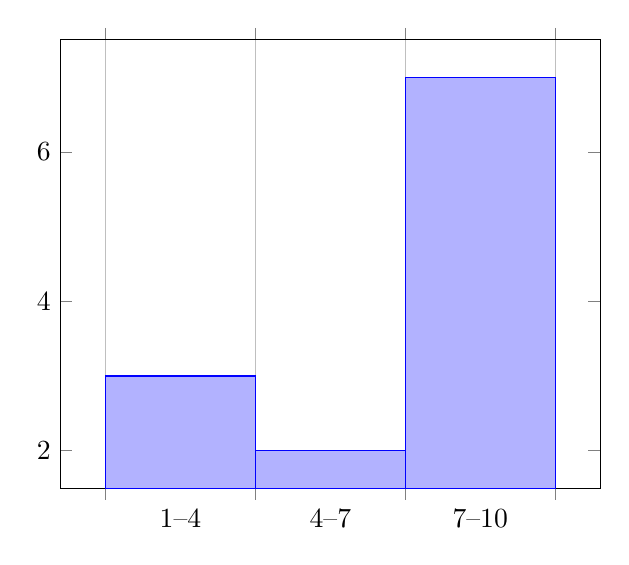
\begin{tikzpicture}
\begin{axis}[
    ybar interval,
    xticklabel=
\pgfmathprintnumber\tick--\pgfmathprintnumber\nexttick
]
    \addplot+ [hist={bins=3}]
        table [row sep=\\,y index=0] {
            data\\
            1\\ 2\\ 1\\ 5\\ 4\\ 10\\
            7\\ 10\\ 9\\ 8\\ 9\\ 9\\
    };
\end{axis}
\end{tikzpicture}
\end{codeexample}
    %
    我们看到 |hist={bins=3}| 接受一列的表作为输入。数据值落入范围 $[1,10]$，
    它被划分为~$3$ 个（等长）区间。最后，绘制落入三个区间各自的点数。
    |xticklabel| 键显示范围（注意它仅与 |x tick label as interval| 配合工作，
    后者已由 |ybar interval| 预先启用）。我们看到范围 $[1,4)$ 内有 $3$ 个元素，
    范围 $[4,7)$ 内有 $2$ 个元素，范围 $[7,10]$ 内有 $7$ 个元素。

    区间是半开区间，即右端点不属于该区间。只有最后一个区间包含其右端点。
    %
\pgfplotsexpensiveexample
\begin{codeexample}[]
\begin{tikzpicture}
\begin{axis}[
    ybar interval,
    xtick=,% reset from ybar interval
    xticklabel={
        $[\pgfmathprintnumber\tick,
         \pgfmathprintnumber\nexttick)$
    },
    x tick label style={draw=red},
]
    % a data file containing 8000 normally distributed
    % random numbers of mean 0 and variance 1
    \addplot+ [hist={data=x}]
        file {plotdata/pgfplots.randn.dat};
\end{axis}
\end{tikzpicture}
\end{codeexample}

    |hist| 图类型也可与 \verbpdfref{plot expression} 组合：像对线图那样提供
    通常的 \meta{expression}。然后根据 |x|、|y| 或 |z| 配置
    |data=|\meta{expression} 的值：
    %
\pgfplotsexpensiveexample
\begin{codeexample}[]
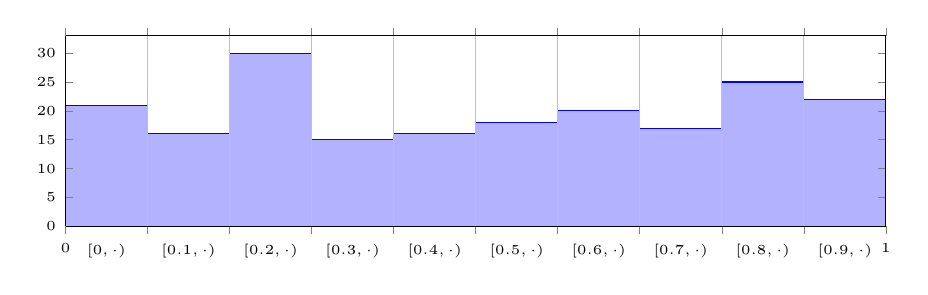
\begin{tikzpicture}
    \begin{axis}[
        tiny,
        height=4cm,width=12cm,
        ybar interval,
        ymin=0,
        xmin=0,xmax=1,
        axis on top,
        extra x ticks={0,1},
        extra x tick style={
            grid=none,
            x tick label as interval=false,
            xticklabel={$\pgfmathprintnumber\tick$}
        },
        xticklabel={$[\pgfmathprintnumber[fixed]\tick,\cdot)$},
    ]
        \addplot+ [samples=200,hist] {rnd};
    \end{axis}
\end{tikzpicture}
\end{codeexample}
    %
    \noindent 本例使用 \pgfname{} 的 |rnd| 方法，它将 |y| 定义为包含 $[0,1]$
    范围内均匀随机数。然后配置 |hist|。注意 |hist| 有默认 |data=y|，因此它使用
    |y| 坐标作为输入。另注意，这里 |x| 值实际上被忽略。|\begin{axis}[...]| 后的
    选项主要用于缩放图形并插入正确界限。插入 |extra x ticks| 方法是为了演示
    如何在不影响整体布局的情况下添加更多刻度标记。注意，|extra x tick style|
    设置 |x tick label as interval=false|，以禁用图其余部分活动的特殊刻度处理。

    以下键配置 |hist|。若它们在 \meta{options} 内提供，可省略通用键前缀
    |hist/|。

    \begin{pgfplotskey}{hist/data=\marg{expression} (initially y)}
        告知 |hist| 如何获取其数据。通常做法是提供一个数学 \meta{expression}，
        它依赖于 |\addplot| 语句提供的数据。例如，若使用 |\addplot expression|，
        \meta{expression} 可依赖 |x|、|y| 或 |z|。对于 |\addplot table| 输入例程，
        \meta{expression} 可使用 |\thisrow|\marg{colname} 访问指定列中当前活动
        的表行。

        也可以避免调用数学解析器。改为使用
        \declareandlabel{hist/data value}|=|\marg{value}。这里，\meta{value}
        应为数值常量。

        初始配置使用通常成为最终 |y| 坐标的值作为输入（更准确地说，初始值为
        |data value=\pgfkeysvalueof{/data|\allowbreak| point/y}|）。
    \end{pgfplotskey}

    \begin{pgfplotskeylist}{%
        hist/data min=\marg{min value} (initially /pgfplots/xmin),
        hist/data max=\marg{max value} (initially /pgfplots/xmax)%
    }
        允许手动提供最小/最大值（即 $\underline m$ 与 $\overline m$）。

        若为空，这些值将从输入数据范围推导。

        所得区间将被划分为 |hist/bins| 个区间。

        初始配置使用任何提供的数据界限，即（自然）选择
        |hist/data min=||xmin| 与 |hist/data max=||xmax|。
    \end{pgfplotskeylist}

    \begin{pgfplotskey}{hist/bins=\marg{number of intervals} (initially 10)}
        指定要使用的区间数。
    \end{pgfplotskey}

    \begin{pgfplotskey}{hist/intervals=\marg{true,false} (initially true)}
        若 |intervals=true|（初始配置），|hist| 将生成 $N+1$ 个坐标，满足
        %
            \[
                \underline m = x_0 < x_1 < \dotsb < x_{N} = \overline m
            \]
        %
        其中 $[\underline m,\overline m]$ 为数据范围。此时，$x_{N-1}$ 与
        $x_N$ 的数据点将获得相同值，即最后一个区间中的元素数。这（仅）在与
        |const plot| 或 |ybar interval| 配合时有用。

        若 |intervals=false|，最后一个数据点将被省略，恰好生成 $N$ 个坐标。
        此时，右端点不显式返回。
    \end{pgfplotskey}

    \begin{pgfplotskey}{hist/cumulative=\marg{true,false} (initially false)}
        允许计算累积直方图。

        累积直方图使用所有先前区间与当前区间之和作为最终值。

        下面是上面的例子，这次带 |hist/cumulative|：
        %
\pgfplotsexpensiveexample
\begin{codeexample}[]
\begin{tikzpicture}
\begin{axis}[
    ybar interval,
    xtick=,% reset from ybar interval
    xticklabel={
        $[\pgfmathprintnumber\tick,
        \pgfmathprintnumber\nexttick)$
    },
]
    % a data file containing 8000 normally distributed
    % random numbers of mean 0 and variance 1
    \addplot+ [hist={data=x,cumulative}]
        file {plotdata/pgfplots.randn.dat};
\end{axis}
\end{tikzpicture}
\end{codeexample}
    \end{pgfplotskey}

    \begin{pgfplotskey}{hist/density=\marg{true,false} (initially false)}
        \textit{由 Jürnjakob Dugge 扩展}
        \vskip\baselineskip
        启用密度估计模式。若 |hist/density| 激活，所得数据点将被重新归一化，
        使总体“质量”等于~$1$。
        %
\pgfplotsexpensiveexample
\begin{codeexample}[]
\begin{tikzpicture}
    \begin{axis}[small,ymin=0,title=\texttt{hist}]
        \addplot [
            hist,
            fill=orange!75,
            draw=orange!50!black]
                table [y index=0] {plotdata/pgfplots.randn.dat};
    \end{axis}
\end{tikzpicture}
%
\begin{tikzpicture}
    \begin{axis}[small,ymin=0, title=\texttt{hist=density}]
        \addplot [
            hist=density,
            fill=orange!75,
            draw=orange!50!black]
                table [y index=0] {plotdata/pgfplots.randn.dat};
    \end{axis}
\end{tikzpicture}
\end{codeexample}


        键 |hist/density| 与 |hist/cumulative| 也可组合：
        %
\pgfplotsexpensiveexample
\begin{codeexample}[]
\begin{tikzpicture}
    \begin{axis}[small,ymin=0, title=\texttt{hist=cumulative}]
        \addplot [
            hist=cumulative,
            fill=orange!75,
            draw=orange!50!black]
                table [y index=0] {plotdata/pgfplots.randn.dat};
    \end{axis}
\end{tikzpicture}
%
\begin{tikzpicture}
    \begin{axis}[small,ymin=0, title=\texttt{hist=\{cumulative,density\}}]
        \addplot [
            hist={cumulative,density},
            fill=orange!75,
            draw=orange!50!black]
                table [y index=0] {plotdata/pgfplots.randn.dat};
    \end{axis}
\end{tikzpicture}
\end{codeexample}
    \end{pgfplotskey}

    \begin{stylekey}{/pgfplots/hist/handler (initially ybar interval)}
        允许更改生成坐标的可视化方式。键 |hist/handler| 是样式，因此使用
        使用 |hist/handler/.style=|\allowbreak|{const plot}| 来更改它。
        %
\begin{codeexample}[]
\begin{tikzpicture}
\begin{axis}
    \addplot+ [
        hist={bins=3},
    ] table [row sep=\\,y index=0] {
        data\\
        1\\ 2\\ 1\\ 5\\ 4\\ 10\\
        7\\ 10\\ 9\\ 8\\ 9\\ 9\\
    };
\end{axis}
\end{tikzpicture}
\end{codeexample}

\begin{codeexample}[]
\begin{tikzpicture}
\begin{axis}
    \addplot+ [
        hist={
            bins=3,
            handler/.style={const plot},
        },
    ] table [row sep=\\,y index=0] {
        data\\
        1\\ 2\\ 1\\ 5\\ 4\\ 10\\
        7\\ 10\\ 9\\ 8\\ 9\\ 9\\
    };
\end{axis}
\end{tikzpicture}
\end{codeexample}

\begin{codeexample}[]
\begin{tikzpicture}
\begin{axis}
    \addplot+ [
        hist={
            bins=3,
            handler/.style={sharp plot},
        },
    ] table [row sep=\\,y index=0] {
        data\\
        1\\ 2\\ 1\\ 5\\ 4\\ 10\\
        7\\ 10\\ 9\\ 8\\ 9\\ 9\\
    };
\end{axis}
\end{tikzpicture}
\end{codeexample}

        注意，|sharp plot| 可能受益于 |intervals=false|：
        %
\begin{codeexample}[]
\begin{tikzpicture}
\begin{axis}
    \addplot+ [
        hist={
            bins=3,
            handler/.style={sharp plot},
            intervals=false,
        },
    ] table [row sep=\\,y index=0] {
        data\\
        1\\ 2\\ 1\\ 5\\ 4\\ 10\\
        7\\ 10\\ 9\\ 8\\ 9\\ 9\\
    };
\end{axis}
\end{tikzpicture}
\end{codeexample}
    \end{stylekey}

    \begin{pgfplotscodekey}{hist/data filter}
        允许定义坐标过滤器，类似于第~\ref{sec:filters} 节所述的坐标过滤器键
        |x filter|。参数 |#1| 是在处理 |hist/data| 后找到的坐标。代码应将
        |\pgfmathresult| 赋值为结果。若之后 |\pgfmathresult| 为空，它将被跳过。
        否则，它应包含一个数字。

        此过滤器在直方图计算\emph{之前}施加。注意，|x filter| 与 |y filter|
        在直方图计算\emph{之后}施加。

        注意，预定义样式如 |each nth point| 也可应用于 |hist/data|，若
        %
        \begin{enumerate}
            \item 在预定义样式名后追加星号 `|*|'，且
            \item 样式的第一个参数为 |hist/data|。
        \end{enumerate}
        %
        例如，|each nth point*={hist/data}{2}| 将跳过 |hist/data| 的第二个输入值
        （试试看）。
    \end{pgfplotscodekey}

    \begin{pgfplotsxycodekeylist}{%
        /pgfplots/hist/data coord trafo,
        /pgfplots/hist/data coord inv trafo%
    }
        这些键的工作方式与 |x coord trafo| 和 |x coord inv trafo| 相同。它们
        分别在直方图求值\emph{之前}施加于 |hist/data| 值，以及在结果值赋值\emph{
       之后}施加。

        注意，|hist| 在可视化其结果\emph{之前}会施加 |hist/data coord inv trafo|。因此，可能也需要为 |x coord trafo| 分配类似变换。

        有关自定义变换的更多信息，见 |x coord trafo| 的文档。
    \end{pgfplotsxycodekeylist}

    \begin{pgfplotskey}{hist/symbolic coords=\marg{list}}
        一个样式，为包含 |hist| 图的坐标轴启用 |symbolic x coords|：
        %
\begin{codeexample}[]
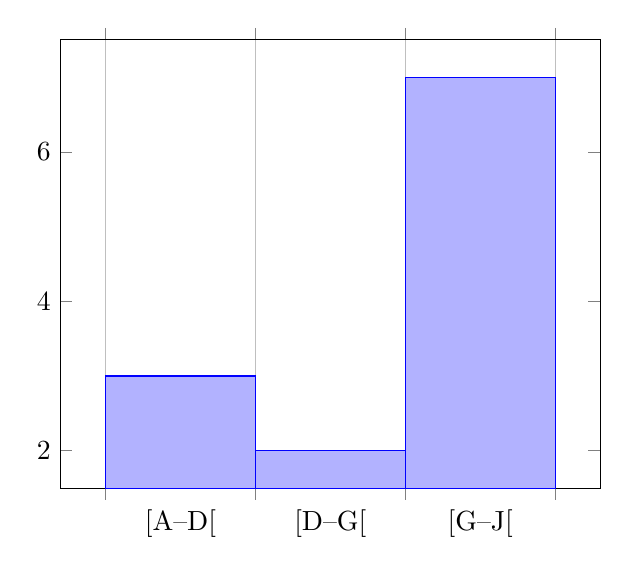
\begin{tikzpicture}
\begin{axis}[
    ybar interval,
    hist/symbolic coords={A,B,C,D,E,F,G,H,I,J},
    xticklabel={[\tick--\nexttick[},
]
    \addplot+ [
        hist={bins=3},
    ] table [row sep=\\,y index=0] {
        data\\
        A\\ B\\ A\\ D\\ F\\ J\\
        G\\ J\\ I\\ H\\ I\\ I\\
    };
\end{axis}
\end{tikzpicture}
\end{codeexample}
        %
        该样式做两件事：首先，它定义 |hist/data coord trafo| 与
        |hist/data coord inv trafo|；然后，它以相同参数调用 |symbolic x coords|。


        \paragraph{注意：}

        当有 |symbolic coords| 时，不要使用 |hist/data=x| 或其他符号值作为输入。
        你需要提供\emph{可展开}值，如 |\pgfkeysvalueof{/data point/x}|
        （效果相同，但直接展开为正确值），而非符号值。

        有关符号坐标的更多细节，请参考 |symbolic x coords| 的文档。
    \end{pgfplotskey}
\end{plottype}
\endgroup
